\documentclass[a4paper,10pt]{article}
\usepackage[utf8]{inputenc}
\usepackage[french]{babel}
\usepackage[T1]{fontenc}
\usepackage{lmodern}
\usepackage{amssymb,amsmath,amsfonts,amsxtra,amsthm}
\usepackage{array}
\usepackage{mathrsfs}
\usepackage{tikz}
\usepackage{graphicx}
\usepackage{caption}
\usepackage{color}
\usepackage{colortbl}
\usepackage{amsmath}
\usepackage{cancel}
\usepackage{subfig}
\usepackage{graphics}
\usepackage{enumerate}
\usepackage[utf8]{inputenc}
\usepackage{a4wide}
\usepackage{amsmath}
\usepackage{verbatim}
\usepackage{array}
\usepackage{clrscode3e}

\begin{document}
	
\section{Analyse descriptive}
\subsection{ }
	
		\begin{center}
			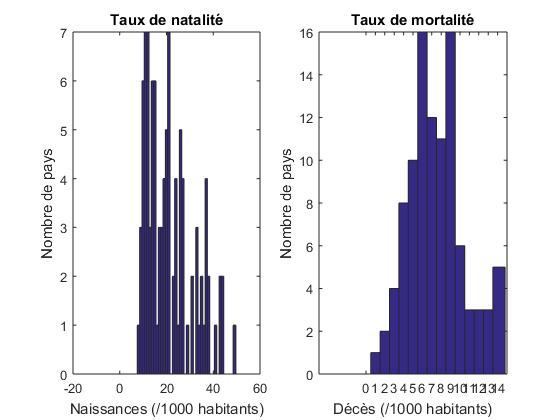
\includegraphics[width=150mm]{Figure1.jpg}
			\captionof{figure}{Population totale}
		\end{center}

Les graphiques ci-dessus classent les taux de natalité et de mortalité en fonction du nombre de pays. La présence de pics plus espacés sur le graphe du taux de natalité montre que l'on trouve des nombres conséquents de pays ayant des taux de natalité différents. En comparaison, un pays sur deux a un taux de mortalité d'entre quatre et huit décès pour mille habitants.

\subsection{ }
Les résultats calculés pour la moyenne, la médiane, le mode et l'écart-type sont les suivants: \\



\begin{tabular}{|l|c|r|}
	\hline
	  & Taux de natalité & Taux de mortalité \\
	\hline
	Moyenne & 21.406  & 7.567 \\
	Médiane & 19.5 & 7 \\
	Mode & 11.6 & 7 \\
	Écart-type & 10.0529 & 2.9361 \\
	\hline
\end{tabular}
\\


Les valeurs représentées pour chaque taux est 11.6 pour le taux de natalité, relevé dans deux pays, et 7 pour le taux de mortalité, que l'on retrouve dans quatre pays
\\
L'écart type élevé pour le taux de natalité montre que les données sont plus dispersées autour de la moyenne alors que celles du taux de natalité tendent vers l'homogénéité. Nous pouvons ajouter à ceci une différence |médiane-moyenne| plus importante pour le taux de natalité.

Les comparaisons avec la Belgique donnent ceci: 

\begin{itemize}
	\item avec 11.7 pour 1000 habitants, le taux de natalité de la Belgique est largement inférieur à la moyenne alors qu'à l'inverse, le taux de mortalité belge, de 9.9 pour 1000 habitants, est supérieur à la moyenne de l'échantillon   
	\item au vu des deux médianes calculées, l'on observe que la Belgique fait partie des pays qui un taux de natalité plus faible et un taux de mortalité plus élevé
	\item on trouve dans l'échantillon deux pays présentant des taux de natalité/mortalité proches de ceux de la Belgique: la Finlande (11.2, 9.4) et la Serbie Montenegro (11.6, 9.5)
\end{itemize}


\subsection{ }

Les taux "normaux" correspondent aux intervalles [11.3531;31.4589] pour le taux de natalité (65 pays) et [4.6309;10.5031] pour le taux de mortalité (70 pays). Il est intéressant de constater que la Belgique se situe dans le voisinage de la borne inférieure du taux de natalité "normal" et dans celui de la borne supérieurs du taux de mortalité "normal". 

\subsection{ }

\begin{center}
	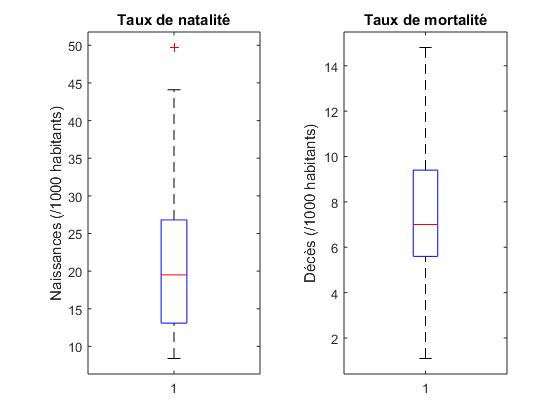
\includegraphics[scale=0.5]{Figure2.jpg}
	\captionof{figure}{Boîtes à moustaches}
\end{center}



Valeurs des quartiles: 
 \begin{itemize}
 	\item Taux de natalité: $Q1=13.1$ et $Q3=26.8$
 	\item Taux de mortalité: $Q1=5.6$ et $Q3=9.4$
 \end{itemize} 

La seule valeur aberrante de l'échantillon est celle correspondant au taux de natalité du Niger, qui est de 49.7/1000 habitants. En effet, ce nombre est supérieur à la valeur donnée par $Q3+1.5*(Q3-Q1)=47.35$.

\subsection{ }

\begin{center}
	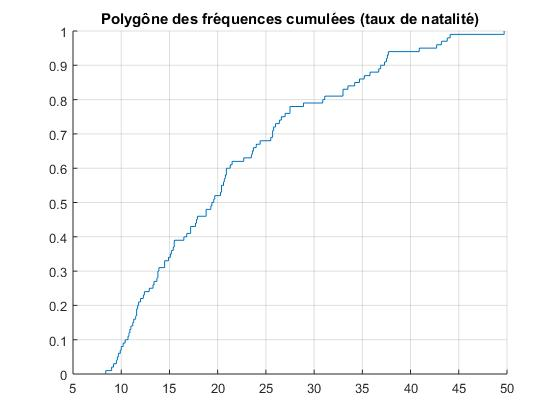
\includegraphics[scale=0.5]{Figure3.jpg}
	\captionof{figure}{Boîtes à moustaches}
\end{center}


Il y a, dans l'échantillon, 32 pays dont le taux de natalité est à la fois inférieur à 20/1000 habitants et supérieur à celui de la Belgique.


\subsection{ }

\begin{center}
	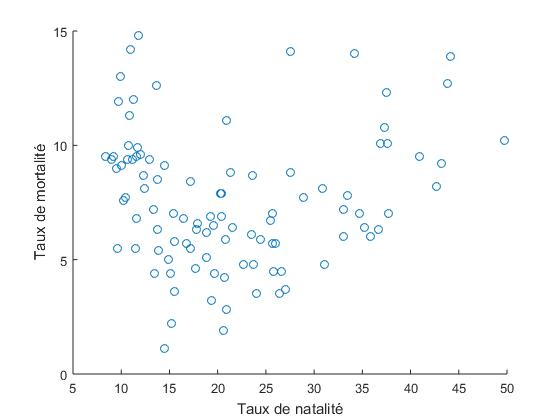
\includegraphics[scale=0.5]{Figure4.jpg}
	\captionof{figure}{Scatterplot}
\end{center}


Le coefficient de corrélation de 0.0676, très faibl, témoigne de l'absence de corrélation entre les deux taux (les pays étant classés par ordre alphabétique). Toutefois il semble que le taux de mortalité augmente graduellement au delà de la médiane du taux de natalité alors qu'il prend des valeurs dans un intervalle plus large lorsque le taux de natalité est inférieur à sa médiane.

\section{Génération d'échantillons i.i.d}

\subsection{Un échantillon i.i.d de 20 pays}

\begin{tabular}{|l|c|r|}
	\hline
	 & Taux de natalité & Taux de mortalité\\
	\hline
	Moyenne & 21.815 &  8.35 \\
	Médiane & 20.05  & 7.75\\
	Écart-type & 9.2549 & 3.215 \\
	\hline
\end{tabular}
\\


Les statistiques descriptives du taux de mortalité de l'échantillon de 20 pays sont toutes plus élevées que celles de la population totale. Il en va de même pour le taux de natalité, à l'exception de l'écart-type, qui est moins élevé dans l'échantillon.


\begin{center}
	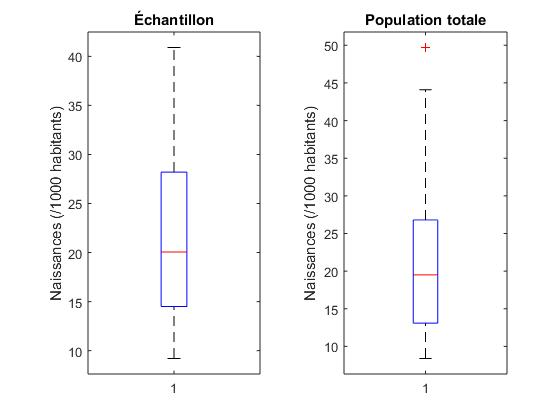
\includegraphics[scale=0.5]{Figure5.jpg}
	\captionof{figure}{Boxplot taux de natalité}
\end{center}


\begin{center}
	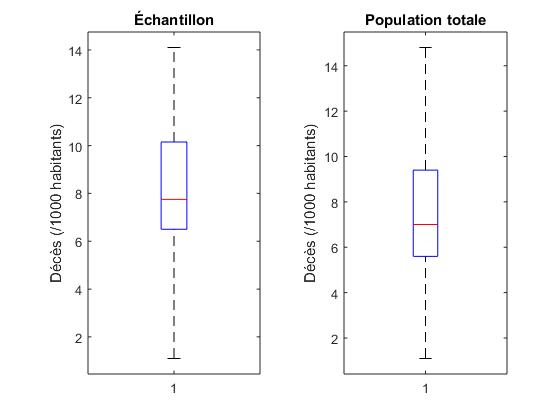
\includegraphics[scale=0.5]{Figure6.jpg}
	\captionof{figure}{Boxplot taux de mortalité}
\end{center}

Caractéristiques de l'échantillon: 

\begin{itemize}
	\item Taux de natalité: valeurs$\in$[9.2;40.9] $Q1=14.5$ $Q3=28.2$
	\item Taux de mortalité: valeurs$\in$[1.1;14.1] $Q1=6.5$ $Q3=10.15$ 
\end{itemize}

La valeur aberrante du taux de natalité n'est plus présente dans la boîte à moustaches de l'échantillon car la valeur donnée par $Q3+1.5*(Q3-Q1)$ est supérieure au taux de natalité maximal de l'échantillon. [8.4;49.7]  [1.1;14.8]


\begin{center}
	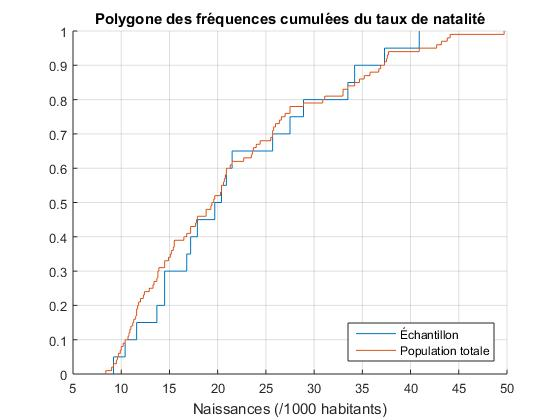
\includegraphics[scale=0.5]{Figure7.jpg}
	\captionof{figure}{Comparaison taux de natalité}
\end{center}

\begin{center}
	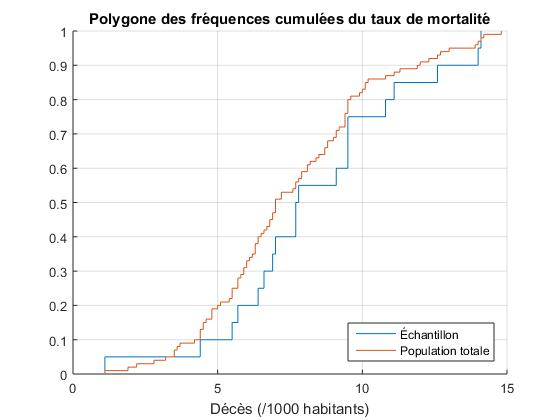
\includegraphics[scale=0.5]{Figure8.jpg}
	\captionof{figure}{Comparaison taux de mortalité}
\end{center}

Les polygones des fréquences cumulées sont relativement semblables pour l'échantillon et la population totale. La distance de Kolmogorov Smirnov est nulle dans les deux cas, preuve du caractère semblable des graphese.


\subsection{500 échantillons de 20 pays}

\begin{center}
	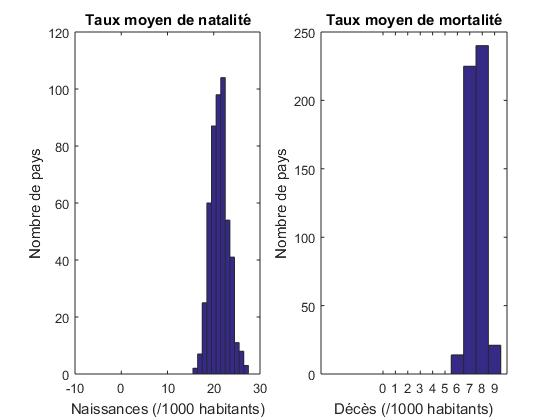
\includegraphics[scale=0.8]{Figure9.jpg}
	\captionof{figure}{Taux moyens}
\end{center}

\begin{itemize}
	\item Moyenne taux de natalité: 21.2455/1000 habitants
	\item Moyenne taux de mortalité: 7.5507/1000 habitants
\end{itemize}

\begin{center}
	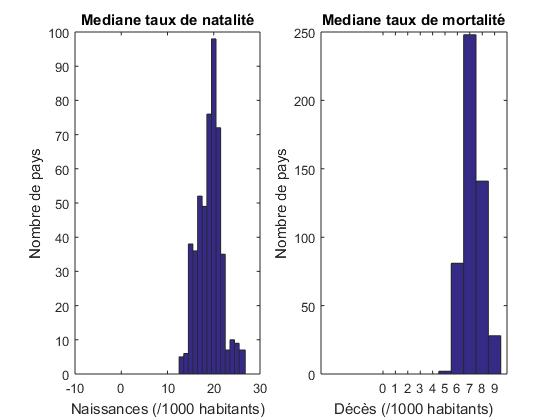
\includegraphics[scale=0.8]{Figure10.jpg}
	\captionof{figure}{Medianes}
\end{center}


\begin{itemize}
	\item Moyenne médiane du taux de natalité: 19.1076
	\item Moyenne médiane taux de mortalité: 7.2476
\end{itemize}


\begin{center}
	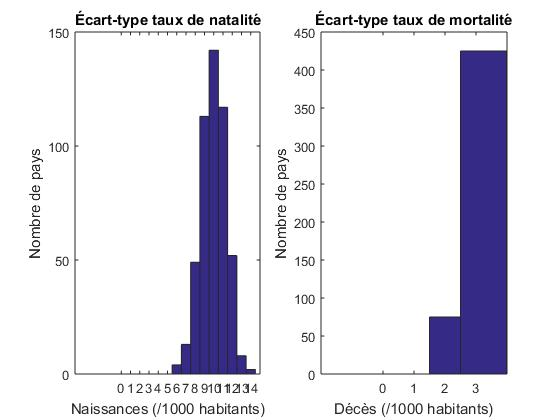
\includegraphics[scale=0.8]{Figure11.jpg}
	\captionof{figure}{Écart-types}
\end{center}


\begin{itemize}
	\item Moyenne écart-type taux de natalité: 9.9622
	\item Moyenne écart-type taux de mortalité: 2.9207
\end{itemize}


Les allures des graphes ci-dessus sont semblables à celles correspondant à une loi normale.

 


\begin{center}
	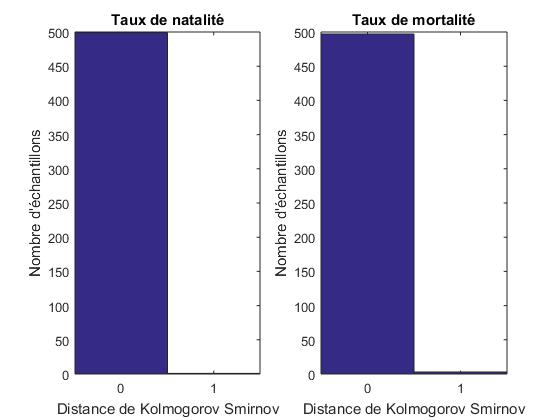
\includegraphics[scale=0.8]{Figure12.jpg}
	\captionof{figure}{Distances de Kolmogorov Smirnov}
\end{center}


Seuls quatre échantillons sur 500 ont une Distance de Kolmogorov Smirnov non nulle pour leur taux de natalité ou de mortalité.

\section{Estimation}

Lorsque la taille des échantillons angmente de 20 à 50, les valeurs des différentes statistiques calculées se rapprochent de zéro.


En utilisant la loi student, aucun intervalle de confiance n'est obtenu alors que l'on obtient 93 intervalles de confiance en utilisant la loi de Gauss

\section{Test d'hypothèse - proportion}


L'hypothèse a été rrejetée par l'État Belge une fois. Pareillement, l'OMS a considéré que les Belges n'ont pas un faible taux de natalité une fois. Mêmes résultats.


Une solution serait de faire en sorte que tout le monde travaille avec les mêmes échantillons.
	
